\subsubsection{Geometry Operations}
\label{sec:geometry_operations}

The geometry menu is triggered by clicking on the respective symbol of the layer.\\

\paragraph{Common Layer Operations}
\begin{figure}[H]
    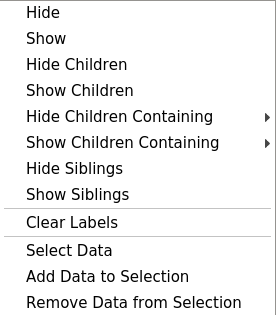
\includegraphics[width=5cm,frame]{figures/geoview_layer_context_menu.png}
  \caption{Geographic View layer context menu}
\end{figure}

\iffalse
 \item Set Color: Open colour dialog to set the items colour
 \item Set Symbol: Set the items symbol to one of the following values:
\begin{itemize}
 \item Cross
 \item Circle
 \item Square
 \item Triangle
\end{itemize}
 \item Set Symbol Size: Set the symbols size
 \item Set Line Width: Set the line width
 \item Set Opacity: Set the items opacity
\fi

\begin{itemize}
 \item Hide: Disable display of this item
 \item Show: Enable display of this item
 \item Hide Children: Disable display of all children
 \item Show Children: Enable display of all children
 \item Hide Children Containing: Disable display of all children containing a specific DBContent
 \item Show Children Containing: Enable display of all children containing a specific DBContent
 \item Hide Siblings: Disable display of all sibling items (children of parent except this one)
 \item Show Siblings: Enable display of all sibling items (children of parent except this one)
 \item Clear Labels: Removes all labels
\end{itemize}

\paragraph{Selection Operations}

\begin{itemize}
 \item Select Data: Select (only) target reports in the group
 \item Add Data to Selection: Add target reports in the group to selection
 \item Remove Data from Selection: Remove target reports in the group from selection
\end{itemize}

\paragraph{ARTAS Target Report Usage Operations}
If ARTAS Target Report Usage information was calculated, and the current layer contains system track updates, the following operations exist:

\begin{itemize}
 \item Show ARTAS Target Report Usage: Shows the target reports used by ARTAS in the group
 \item Clear ARTAS Target Report Usage: Hides the target reports used by ARTAS in the group
\end{itemize} 


\paragraph{Ground Lines Operations}
If height information is used, the following operations exist:

\begin{itemize}
 \item Show Ground Lines: Shows the connection lines to the ground for all target reports in the group.
 \item Clear Ground Lines: Clears the connection lines to the ground for all target reports in the group.
\end{itemize} 


\paragraph{Ground Speed Vector Operations}
If ground speed information is loaded (see \nameref{sec:others_ground_speed}), the following operations exist:

\begin{itemize}
 \item Show Ground Speed Vectors: Shows ground speed vectors for all target reports in the group.
 \item Clear Ground Lines: Clears ground speed vectors for all target reports in the group.
\end{itemize} 

\paragraph{Position Accuracy Ellipses Operations}
If position accuracy information is loaded (see \nameref{sec:others_position_accuracy}), the following operations exist:

\begin{itemize}
 \item Show Position Accuracy Ellipses: Shows position accuracy ellipses for all target reports in the group.
 \item Clear Position Accuracy Ellipses: Clears position accuracy ellipses for all target reports in the group.
\end{itemize} 

\paragraph{Special Root Geometry Layer Operations}
This layer has special operation present:

\begin{itemize}
 \item Reset All Styles: Sets all style information to default (including make all data visible)
 \item Clear All Assocations: Removes display of all shown associations of all data
\end{itemize} 
